\documentclass{book}

\input{../activities-preamble.tex}
\begin{document}
\setcounter{project}{172}
\addtocounter{project}{-1}
\begin{activity}[]\label{act-lowerpaths}
\hypertarget{p-1017}{}%
We have already seen how to count lattice paths in \hyperref[act-latticepaths]{Activities~\ref{act-latticepaths}} and \hyperref[act-latticepaths2]{\ref{act-latticepaths2}}.  Now consider a variation.%
\par
\hypertarget{p-1018}{}%
How many paths of length \(2n\), consisting of horizontal and vertical segments of unit length, are there from \((0, 0)\) to \((n, n)\) such that the path never goes above the line \(y = x\)? One such path to \((3, 3)\) is shown in \hyperref[catalanpathex]{Figure~\ref{catalanpathex}}.%
\begin{figure}
\centering
{
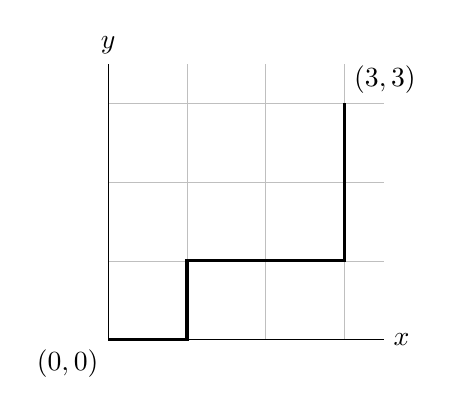
\begin{tikzpicture}
  \draw[very thin, color=gray!50] (0,0) grid (3.5, 3.5);
  \draw[thin] (0,0) -- (3.5,0) node[right]{$x$} (0,0) -- (0,3.5) node[above]{$y$};
  \draw (0,0) node[below left]{$(0,0)$} (3,3) node[above right] {$(3,3)$};
  \draw[very thick] (0,0) -- (1,0) -- (1,1) -- (3,1) -- (3,3);
\end{tikzpicture}
}
\caption{One of the acceptable lattice paths from \((0,0)\) to \((3,3)\).\label{catalanpathex}}
\end{figure}
\par\smallskip%
\noindent\textbf{Solution.}\hypertarget{solution-92}{}\quad%
\hypertarget{p-1019}{}%
Using R for right and U for up, the sequence R U R R U U gives the path. The bijection matching R with H and U with D links paths to H-D sequences.%
\end{activity}
\end{document}
